\chapter{Spectrum sensing}

Spectrum sensing is the main task in the entire operation of cognitive
radio. Spectrum sensing is defined as the finding of spectrum holes in 
the local neighborhood of the cognitive radio receiver. Spectrum holes are the
underutilized (in part or in full) subbands of spectrum at a particular time
in a specific location. Moreover for cognitive radio to fulfil its potential
in solving the problem of spectrum underutilization, the spectrum sensing 
method used should be reliable and computationally feasible in real-time 
\cite{haykin09}.

There are many spectrum sensing techniques available. Three important ones of
them are as follows:
\begin{itemize}
    \item Energy detection
    \item Matched filter detection
    \item Cyclostationarity detection
\end{itemize}

\section{Energy detection}

Conventional energy detector is made up of a low pass filter, an A/D 
converter, a square law detector and an integrator (Figure 
\ref{energyDetection}a). This implementation is not flexible enough, 
especially in the case of narrowband signals and sinewaves. Also, this 
requires a pre-filter matched to the bandwidth $B$ of the signal to be scanned
\cite{cabric06}.

So, an alternative implementation is generally used where we find the squared 
magnitude of the FFT using the Average Periodogram method (Figure 
\ref{energyDetection}b). In this architecture, we can alter the bandwidth of
frequencies scanned just by taking
the required number of FFT bins. 

Spectrum sensing can be viewed as a binary hypothesis-testing problem 
\cite{zhang09}:
\begin{itemize}
    \item $H0$: primary user is absent
    \item $H1$: primary user is present
\end{itemize}

The detection is basically to decide between the following two hypotheses,
\begin{align}
    x(t) &= n(t), & H0 \nonumber \\
    x(t) &= h(t)s(t) + n(t), & H1 \nonumber
\end{align}

where $x(t)$ is the received signal, $s(t)$ is the primary user signal, $h(t)$
is the complex channel gain and $n(t)$ is the additive white gaussian noise
(AWGN) with zero mean and variance $\sigma_n^2$. Generally $h(t)$ is assumed
to be constant $h_0$ for the detection period. A statistics $Y$ is computed by
taking energy samples over a time $T$ in a bandwidth $B$ and compared with a 
predefined threshold $\gamma$ for making the decision.

Energy detection is one of the simplest methods of spectrum sensing. It is the 
optimal detection method for unknown signals. Moreover, it is widely used 
because its computationally less resource-intensive.

\begin{figure}
    \centering
    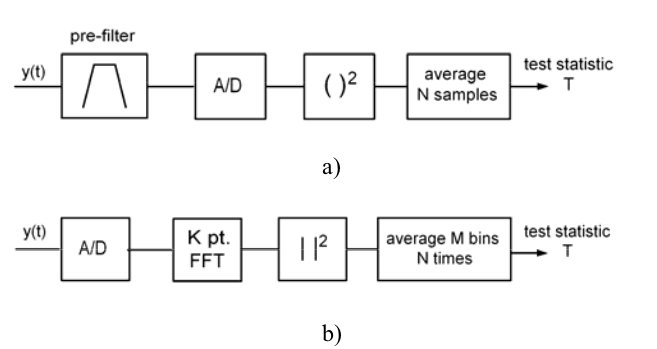
\includegraphics[width=0.7\textwidth]{energyDetection}
    \caption[Energy Detection block diagram]{(a) Implementation using analog 
    filter and square law device \\
    (b) Implementation using periodogram. \\
    \footnotesize{Source: \cite{cabric06}}}
    \label{energyDetection}
\end{figure}

But this method is not without problems. It is always to difficult to 
determine a threshold that will work for all situations. This method cannot
say whether an interfering signal is from a primary user or a secondary user.
Low SNR (signal to noise ratio) signals cannot be detected easily.

The frequency resolution can be improved by increasing N, the number of FFT 
points, but then this requires more samples and thereby takes more time.

\section{Matched filter detection}
A matched filter is a linear filter to maximize the output SNR of a received 
signal. It is the optimum filter to detect signals that are known a priori 
\cite{wikiMF}.


In matched filtering, the received signal is first band pass filtered and then
convolved with the impulse response. The impulse response $h$ here is the 
reference signal itself \cite{bhatta11}. Matched filtering is so called 
because the impulse response is matched to the reference signal.
\begin{equation*}
    Y[n] = \sum_{-\infty}^{\infty} h[n-k]x[k]
\end{equation*}

Here, $x[k]$ is the received or unknown signal with additive noise.
The goal of matched filtering is to enhance the component of reference signal
in the received signal and to suppress the noise. This works best when the 
additive noise is completely orthogonal to the reference signal or when the
noise is completely Gaussian. In practice though, the noise doesn't turn out 
to be purely Gaussian.
 
Matched filtering requires only $O$(1/SNR) samples to meet a given $P_d$, 
probability of detection requirement. Thus it requires less detection time.

But, matched filtering requires us to have a priori information about the 
received signal. This technique requires demodulating the received signal. For
demodulation, we require information like bandwidth, operating frequency, 
modulation type, pulse shaping, packet format, etc. Demodulating the received
signal correctly also requires timing synchronization, carrier 
synchronization, etc. It might still be possible to achive this because the
received data carry preambles, synchronization data, etc.

This method requires a specific type of receiver for every primary user.
Implementing this method on a receiver will increase the complexity and the 
power consumption greatly.

\begin{figure}
\centering
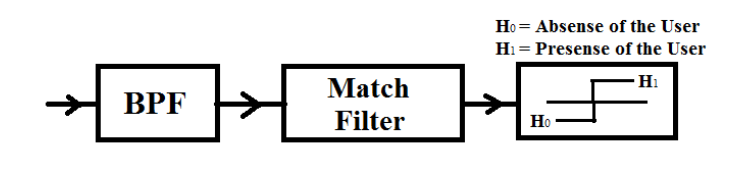
\includegraphics[width=0.8\textwidth]{matchedFilter}
\caption[Matched filter]{Block diagram of Matched filter implementation.}
\label{matchedFilter}
\end{figure}

\section{Cyclostationarity detection}

To identify signals in the presence of noise and other signals, 
cyclostationarity detection uses the periodic properties of the signal. 
Sinusoidal waves, hopping sequences, cyclic prefixes, etc. of primary signals
carry periodic properties in them. These cyclostationary signals manifest 
spectral correlation and other periodic statistics while stationary noise and
interference do not.

These periodic properties are intentionally put in these signals to help the
receivers do timing synchronization, phase synchronization,
direction of arrival estimation \cite{kranthi13}, etc. These periodic 
properties help in identifying some random signal with particular modulation
types even in the midst of noise and interference from other signals.

In low SNR regions, cyclostationarity detection performs better than energy 
detection in identifying or detecting signals. Cyclostationarity detection is
very resistant to noise and other interferences. Although it requires some
a priori information, cyclostationarity can distinguish some Cognitive Radio
signals from primary signals.

The cons of cyclostationarity detection are that it is quite complicated 
mathematically, more computationally involved and requires longer observation
time.

We can detect a signal, given we know its cyclic frequency, by finding that
frequency in the SCD (Spectral Correlation Density) function calculated for 
the received signal. The SCD is also known as CS (Cyclic Spectrum) and SCF 
(Spectral Correlation Function).The SCD is given by \cite{deepa10}:
\begin{equation*}
    S_{x}^{\alpha}(f) = \int_{-\infty}^{\infty}R_{x}^{\alpha}(\tau)e^{-i2\pi 
    f\tau}d\tau
\end{equation*}

where the cyclic autocorrelation function $R_{x}^{\alpha}(\tau)$ is defined as
\cite{gardner91}

\begin{equation*}
    R_{x}^{\alpha}(\tau) {\buildrel\triangle\over =} \lim_{T\rightarrow\infty}
    \int_{-T/2}^{T/2}x(t+\tau/2)x^{\ast}(t-\tau/2)e^{-{i2\pi\alpha t}}dt
\end{equation*}
where $x(t)$ is the received signal and $\alpha$ is the 
\emph{cyclic frequency}.

\begin{figure}
\centering
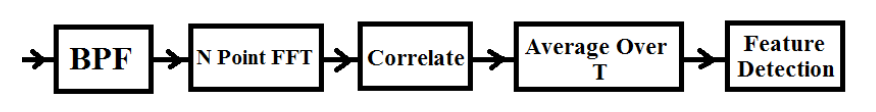
\includegraphics[width=0.7\textwidth]{csd}
\caption[Cyclostationary Detection implementation]{Block diagram 
of Cyclostationary Detection implementation.}
\label{csd}
\end{figure}

We can also get the SCD function by considering a zero mean signal $x(t)$
whose time varying autocorrelation function $R_x(t,\tau)$ defined as
\cite{prithvi11}
\begin{equation*}
    R_{x}(t,\tau) = E\{x(t)x^{\ast}(t+\tau)\}
\end{equation*}

is periodic in time $t$ and can be represented as a Fourier series
\begin{equation*}
    R_{x}(t,\tau) = \sum_{\alpha}R_{x}^{\alpha} (\tau)e^{i2\pi\alpha t} 
\end{equation*}
for which the cyclic autocorrelation function is defined as
\begin{equation*}
    R_{x}^{\alpha}(\tau) = \lim_{T\rightarrow\infty} {\frac{1}{T}}
    \int_{\frac{T}{2}}^{\frac{T}{2}}R_{x}(t,\tau)e^{-i2\pi\alpha t}dT
\end{equation*}
Again the Fourier transform of $R_{x}^{\alpha}(\tau)$ is the SCD defined as
\begin{equation*}
    S_{x}^{\alpha}(\tau)=\int_{-\infty}^{\infty}R_{x}^{\alpha}
    (\tau)e^{-i2\pi f\tau}d\tau
\end{equation*}
Cyclic Spectrum is a two-dimensional transform whereas Power Spectral Density
(PSD) is just one-dimensional. Cyclostationarity detection won't work without
a priori information. But if we have all the a priori information, then 
matched filtering turns out to be a much simpler and faster technique.

\section{Comparison of sensing techniques}

\begin{figure}
\centering
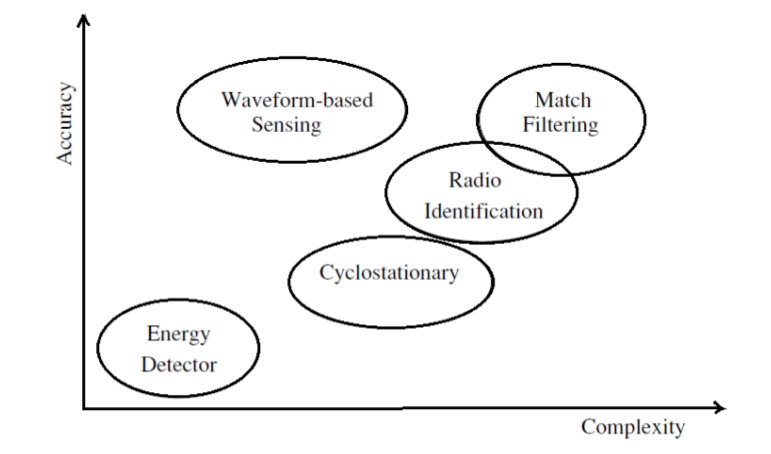
\includegraphics[width=0.77\textwidth]{compareSensing}
\caption[Comparison of sensing methods]{Comparison of some spectrum sensing 
methods}
\label{compareSensing}
\end{figure}

Energy detection technique is the simplest method of all but it is also the 
most error prone. On the other hand, matched filtering is the most complex but 
it is very accurate. Cyclostationarity detection is more complicated than 
energy detection but it is more accurate. There is no ideal detection method.
There are always compromises and tradeoffs to be made. Figure 
\ref{compareSensing} shows a comparison of some spectrum sensing methods.

There are other methods of spectrum sensing that are more involved. For
example multitaper spectral estimation, wavelet based detection, waveform
based detection, etc.


\section{Implementation of energy detection technique}

In this section, we give a brief mathematical overview of the Average 
Periodogram Analysis method, that we have used in this project for energy
detection spectrum sensing. We also dwell on the wideband spectrum analyzer 
which uses Average Periodogram Analysis.

\subsection{Average periodogram analysis}

